\documentclass{article}
\usepackage{amsmath} %This allows me to use the align functionality.
                     %If you find yourself trying to replicate
                     %something you found online, ensure you're
                     %loading the necessary packages!
\usepackage{amsfonts}%Math font
\usepackage{graphicx}%For including graphics
\usepackage{hyperref}%For Hyperlinks
\usepackage{listings}
\lstset{
    numbers=left,
    backgroundcolor = \color{lightgray},
    breaklines=true,
    tabsize=2,
    basicstyle=\ttfamily,
    literate={\ \ }{{\ }}1
}
\usepackage{fancyvrb}
\usepackage{graphicx}
\usepackage{natbib}        %For the bibliography
\bibliographystyle{apalike}%For the bibliography
\usepackage[margin=1.0in]{geometry}
\usepackage{float}
\usepackage{tikz}
\usetikzlibrary{trees}
\begin{document}
%set the size of the graphs to fit nicely on a 8.5x11 sheet
\noindent \textbf{Caio Brighenti }\\
\noindent \textbf{COSC 302 - Analysis of Algorithms -- Spring 2019}\\%\\ gives you a new line
\noindent \textbf{Lab 10}\vspace{1em}\\
\\ \textbf{Required problems:}
	   \begin{center}
	   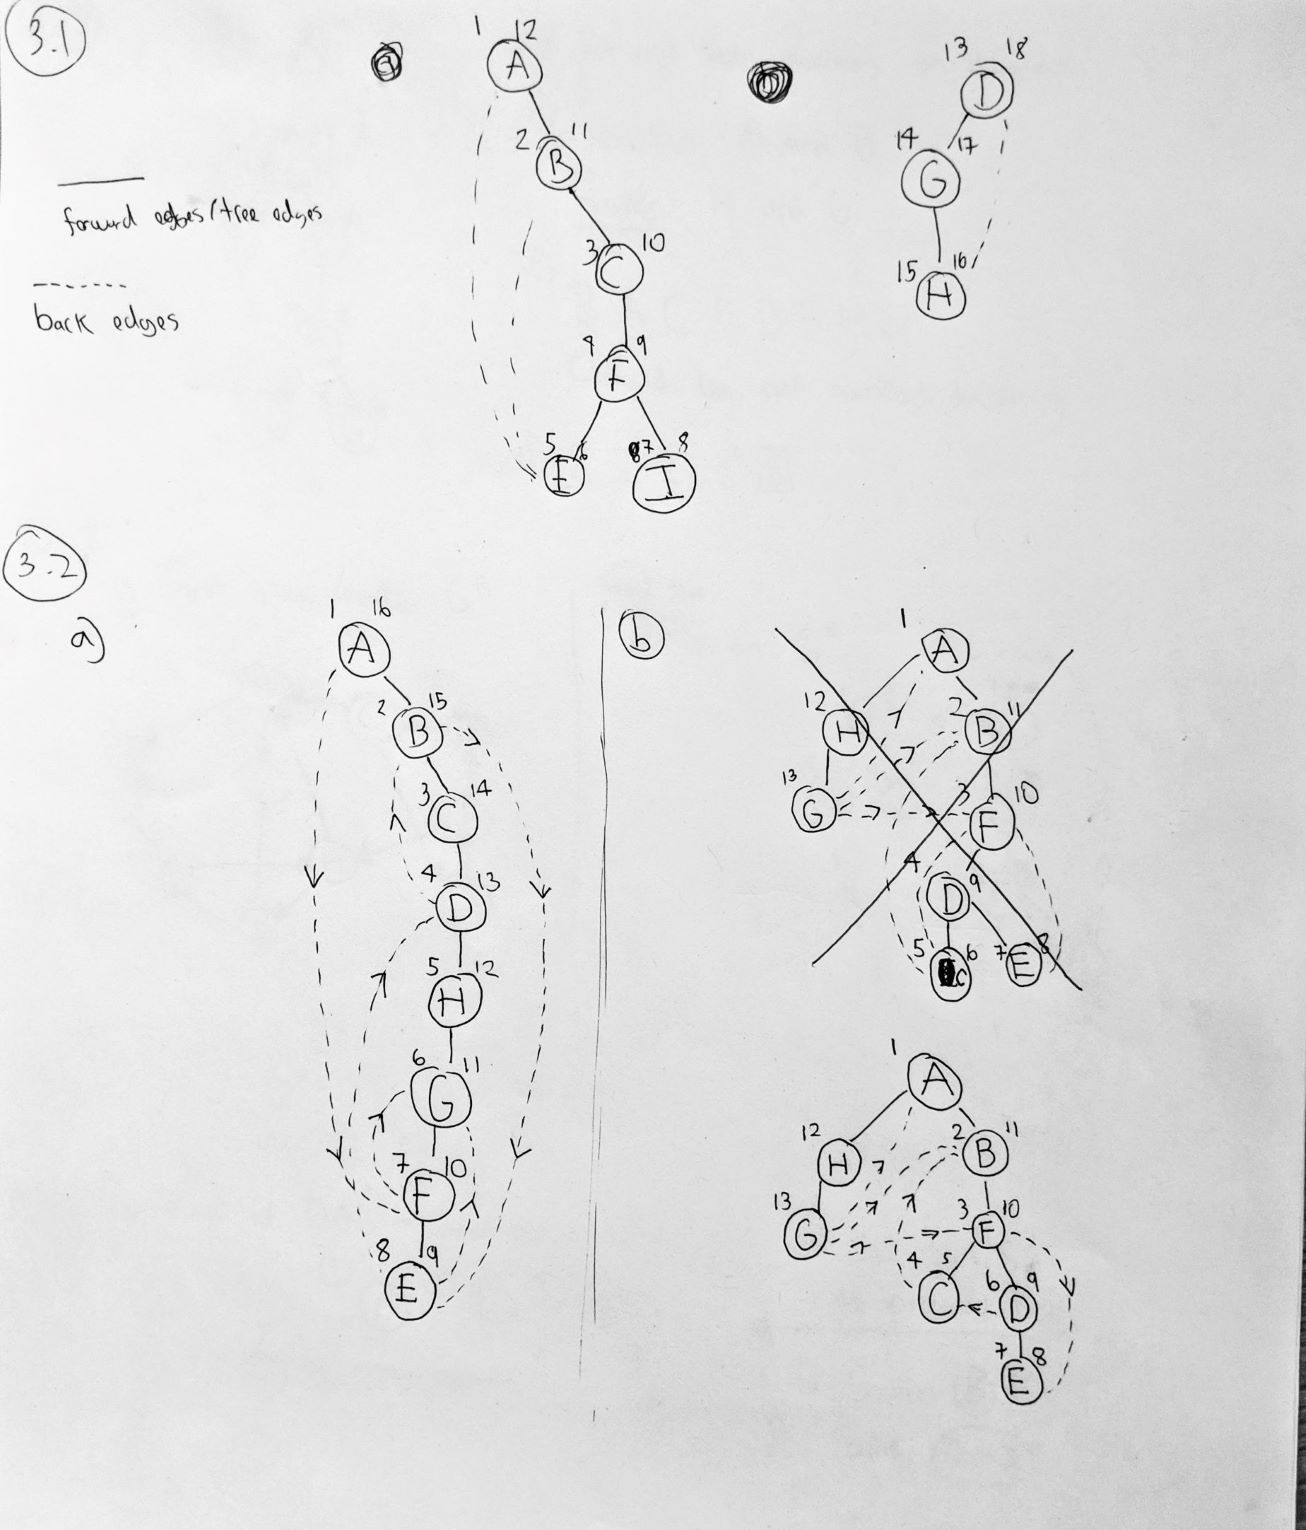
\includegraphics[scale=0.28]{1.jpg} \\
	   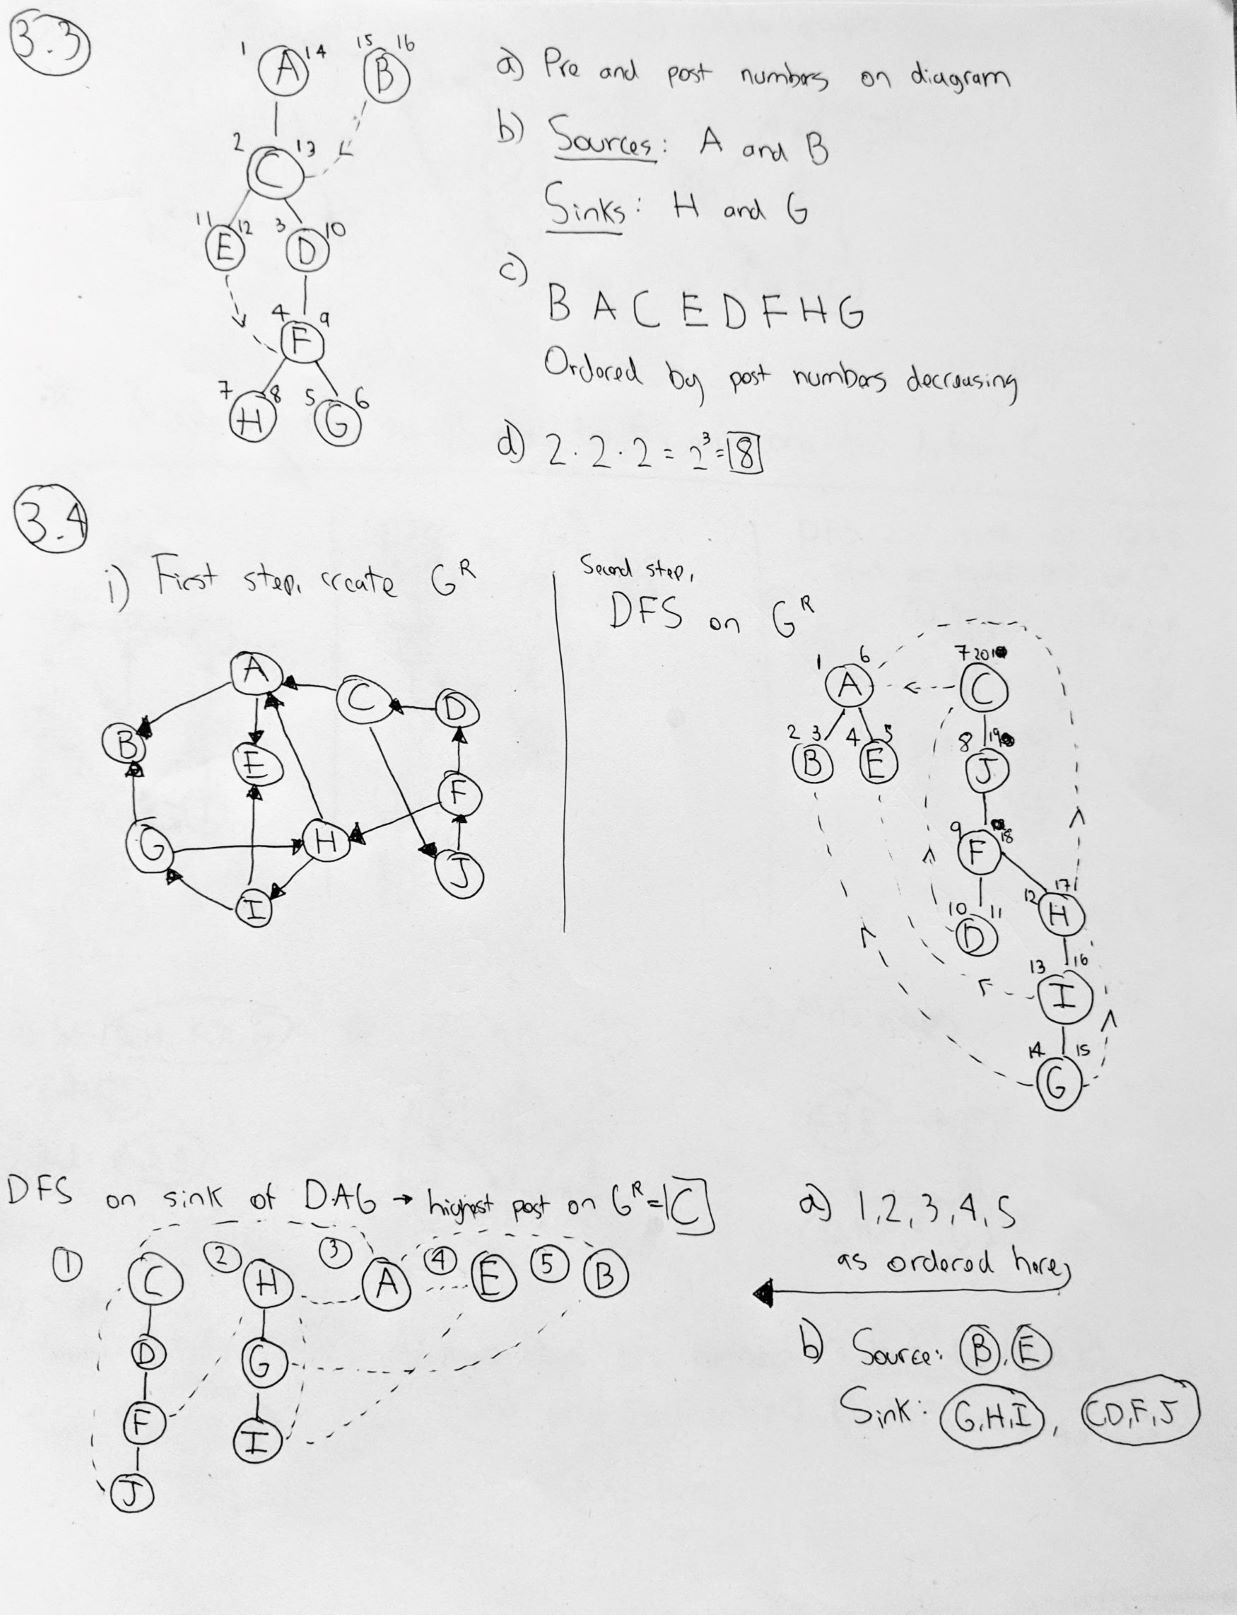
\includegraphics[scale=0.28]{2.jpg} \\
	   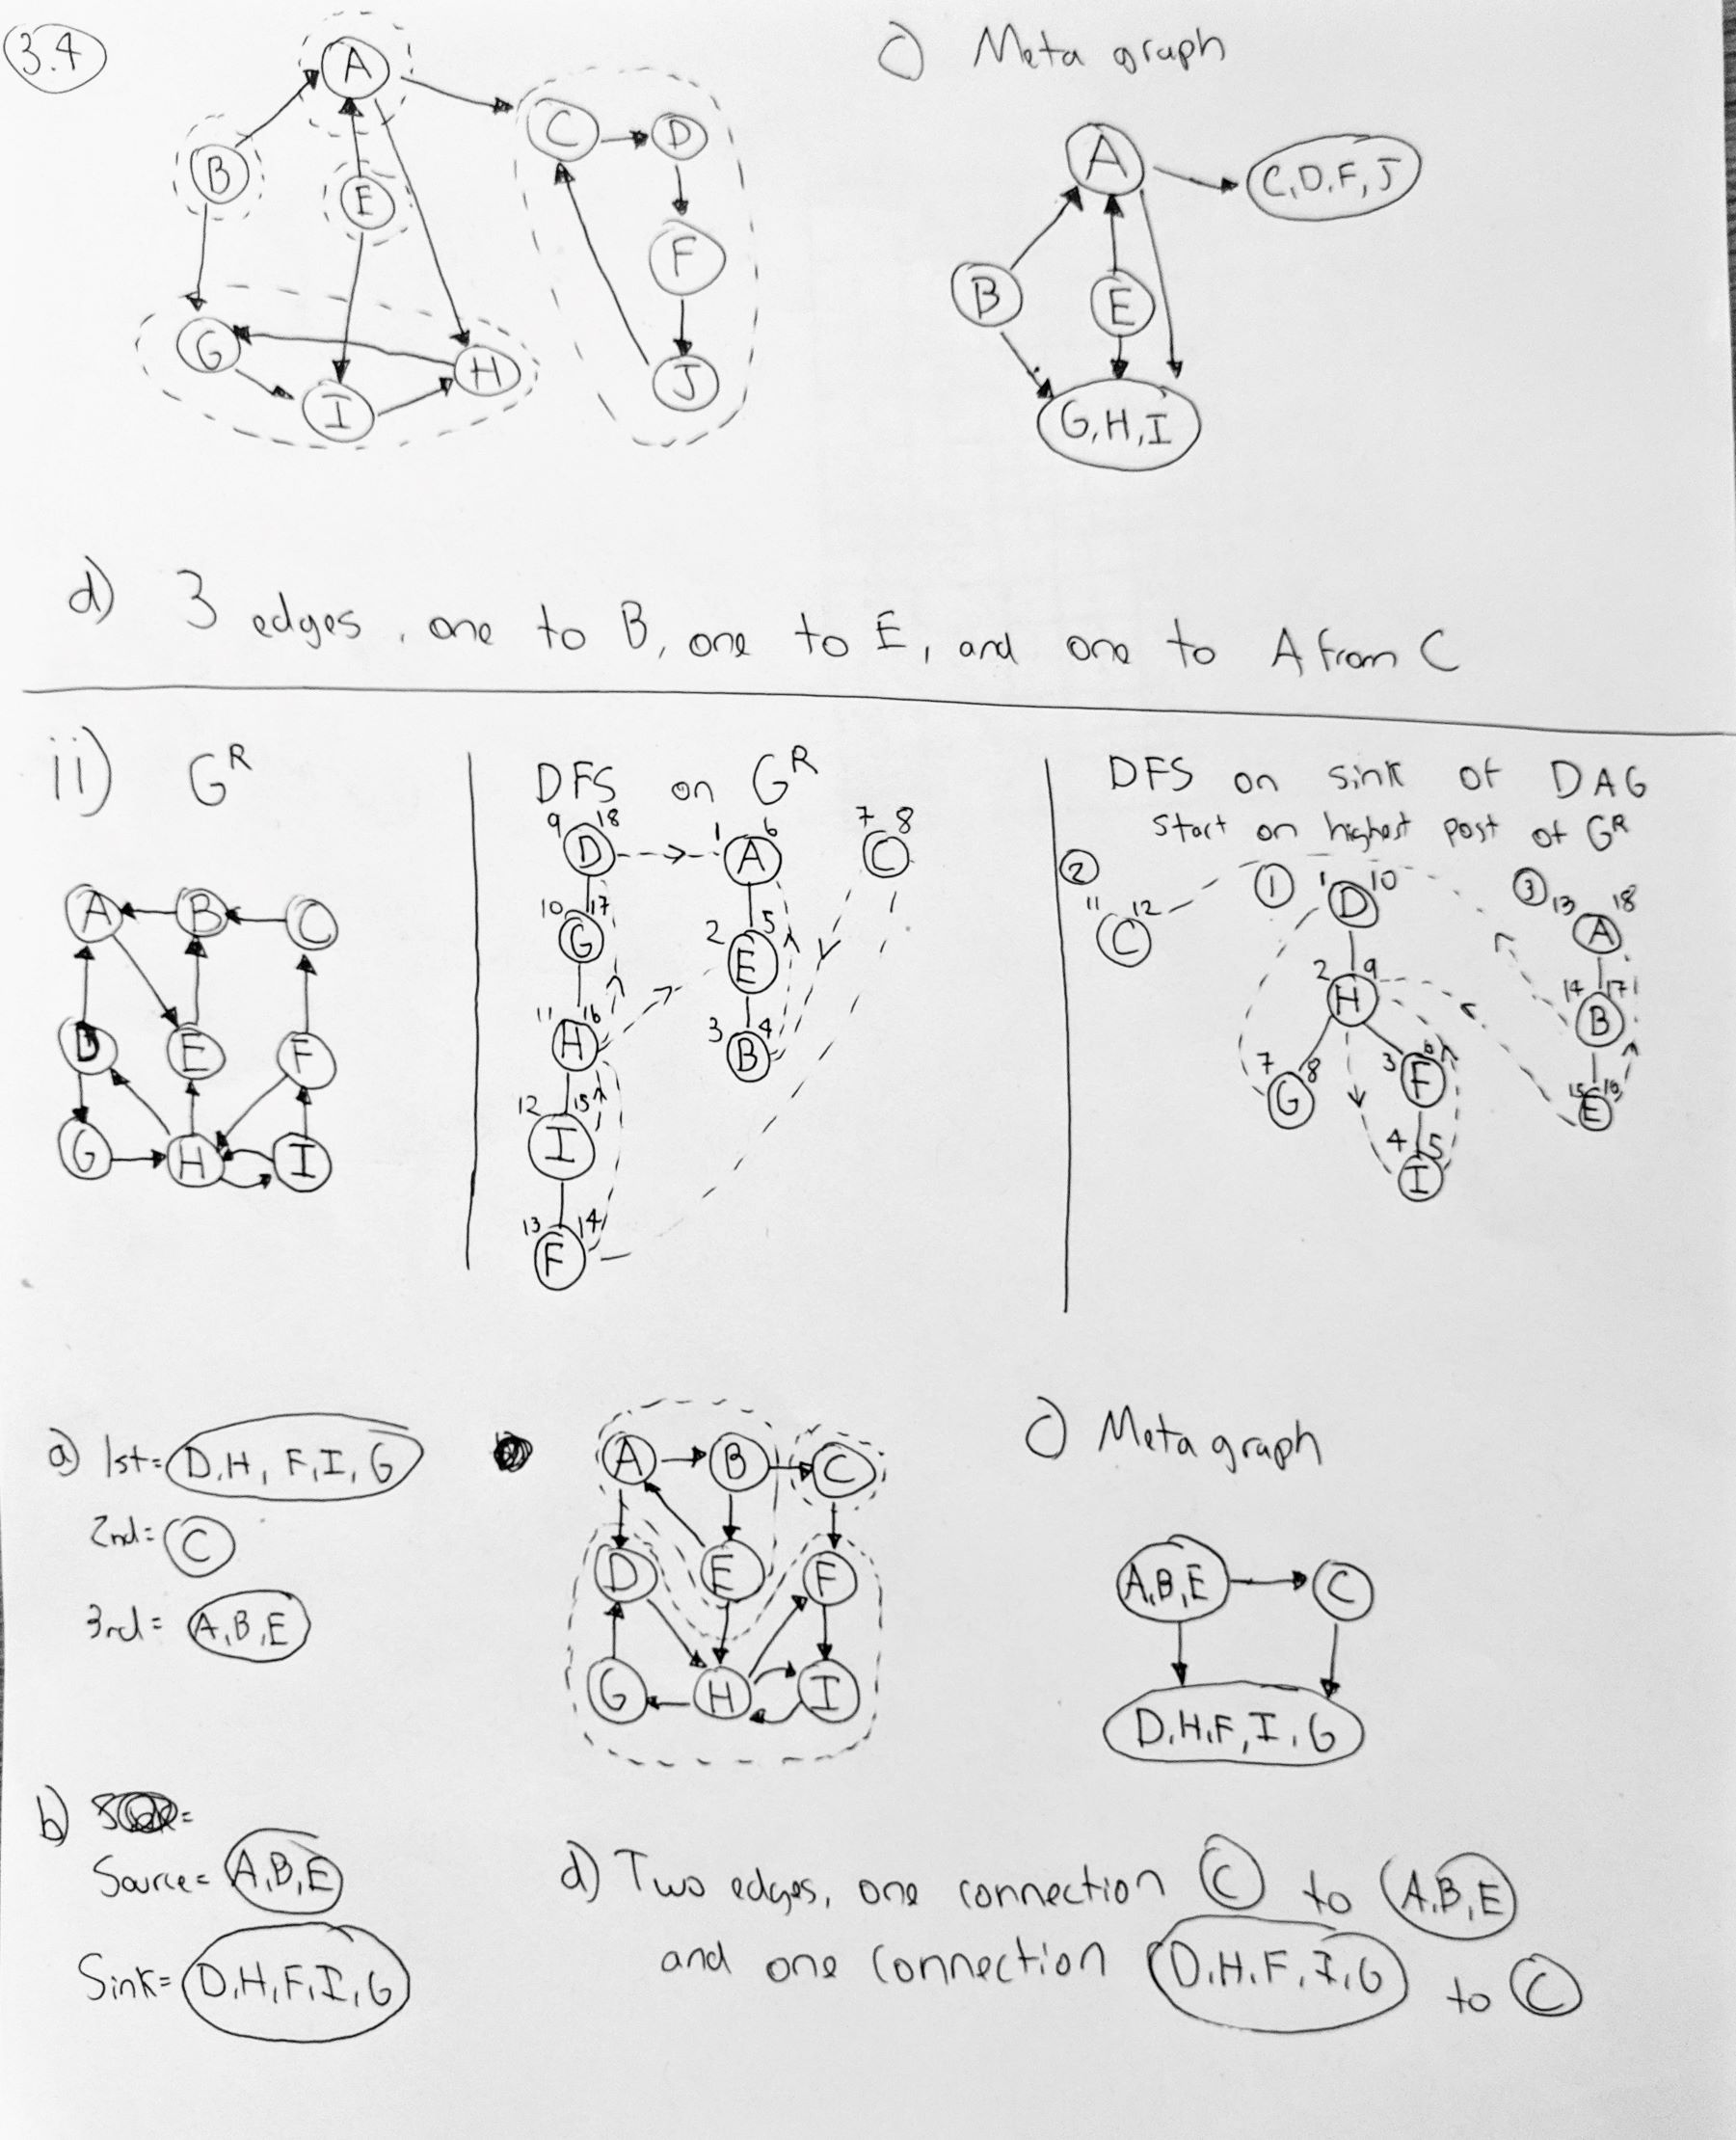
\includegraphics[scale=0.28]{3.jpg} \\
	   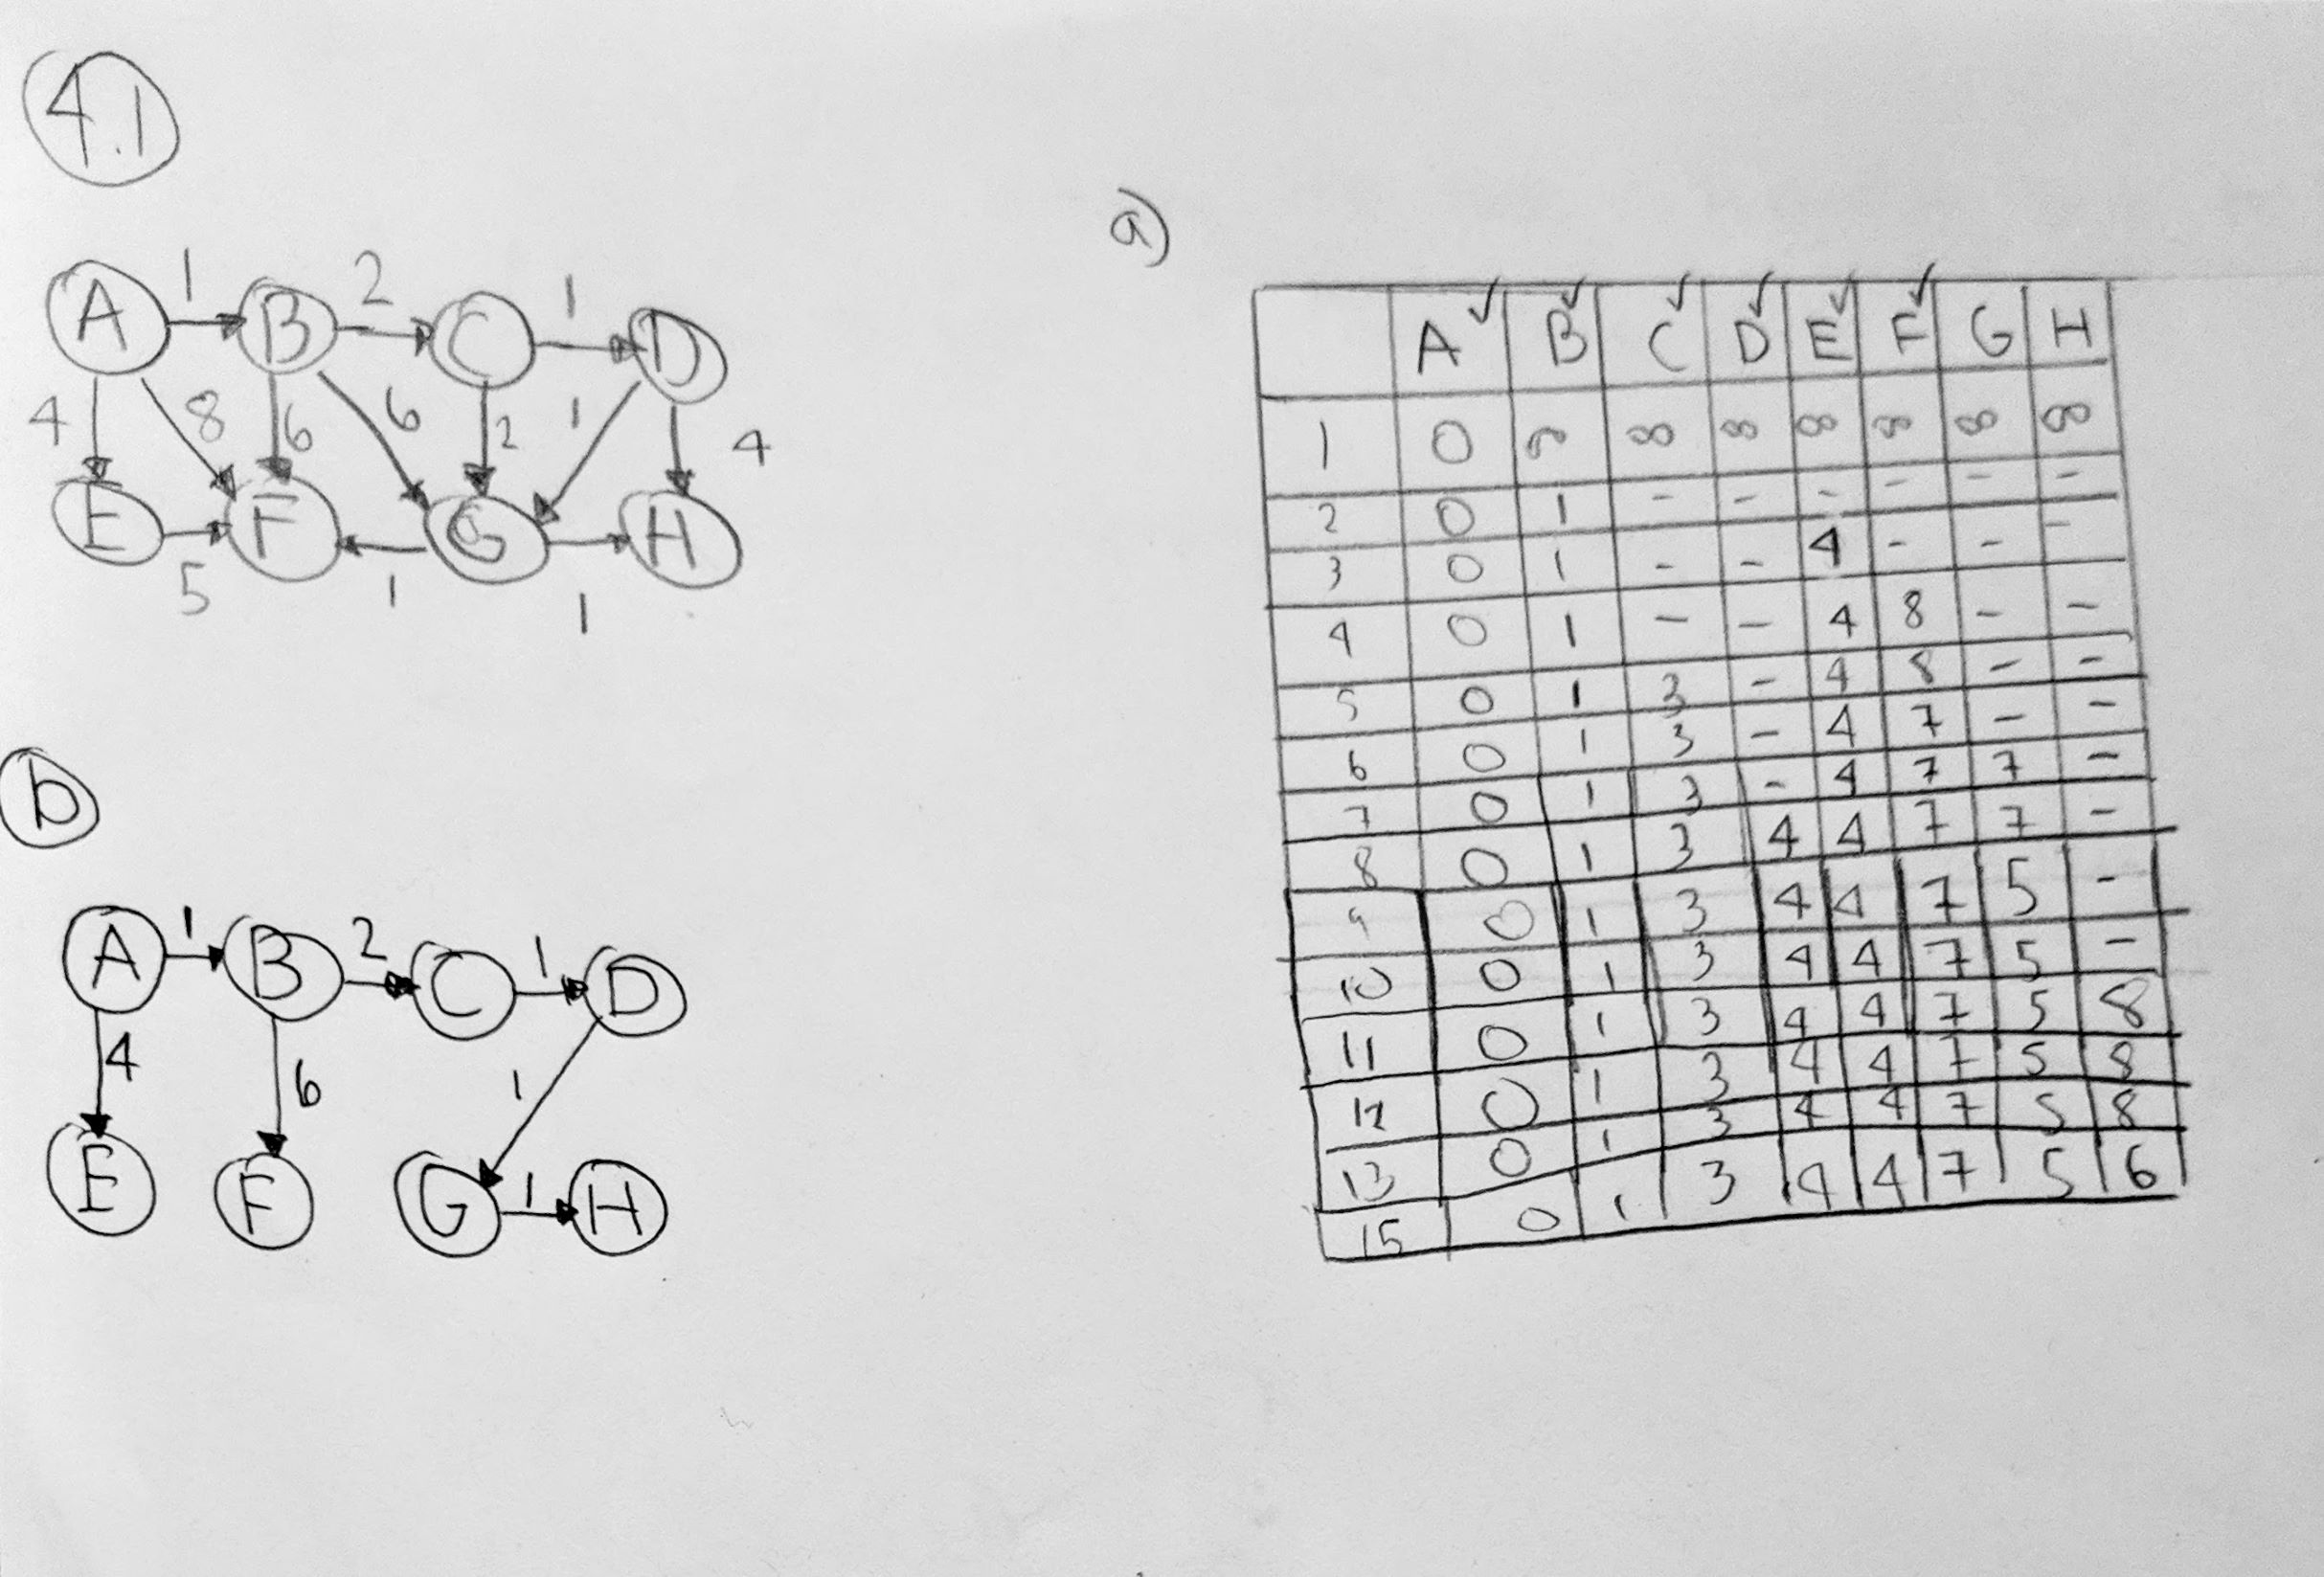
\includegraphics[scale=0.2]{4.jpg} \\ 
	   \end{center}
 \textbf{My assigned problem"}
\begin{enumerate}
	\setcounter{enumi}{7}
	\item \textbf{Problem 4-6}
\\ We must show that the \emph{prev} data structure as created by Dijkstra's algorithm provides us with a tree. We will show this by defining the formal properties of a tree, then showing that each of them holds in the case of \emph{prev}. First, we formally define \emph{prev}. 
\\\\ \textbf{Formal properties of \emph{prev}}
\\ The second textbook defines \emph{prev} as an array that for each node $u$ holds the identity of the node immediately before it on the shortest path from $s$ to $u$. In this case, $s$ is the initial node that Dijkstra's algorithm is called on, and $u$ is any other node on that graph. 
\\ There is one special case in this array. It is plain to see that $s$ would have no node immediately preceding it in a path from $s$, as it is the start of the path. Thus, we consider that $s$ is it's own preceding node. We can also assume that the behavior of \emph{prev} is undefined for a node not in the graph or not reachable from $s$. Next, we outline the formal definition of a tree.
\\ \\ \textbf{Definition of a tree}
\\ Neither textbook includes a formal definition of a simple tree, so I turned to Wikipedia. Wikipedia explains a tree as a non-linear data structure composed of nodes $u$, in which the function $parent(u)$ returns the ancestor of that node. Each non-empty tree also has a root node, for which the function $parent(u)$ returns the root node.
\\ While this is the simple definition, there are a few other properties which must be outlined. Firstly, each node must only have a single parent, but multiple nodes can share the same parent. Alternatively, no two nodes can share the same child, but any node can have any number of nodes. Note that this is not the case in a binary tree, but here we consider the most general case. Additionally, all nodes in the tree must be connected, and reachable in a traversal starting from the root node. Finally, a tree, unlike a graph, may not have any cycles. That is to say, a node cannot have an ancestor as it's child. We distill all of this into three clear properties that define a tree.
\begin{enumerate}
\item Each node $u$ has a \emph{single} parent, and the root has itself as a parent.
\item All nodes are connected and reachable from the root
\item The tree includes no cycles
\end{enumerate}
We individually show that each of these properties holds for the array $prev$. It is important to note that we assume the behavior of Dijkstra's works as expected, outputting $prev$ as the algorithm defines.
\\ \\ \textbf{Property A}
\\ We first show that all nodes have exactly one parent in the array $prev$. As we defined above, $prev(u)$ for any nodes in the graph searched always returns the node immediately preceding it in the path from $s$. Thus, there is only a single output for any input $u$, and consequently only one parent per node. We have also defined that for the node $s$, the starting node, $prev$ returns $s$, which appropriately matches the defined behavior of the root node. Thus, the first property is met.
\\ \\ \textbf{Property B}
\\ We show that all nodes $u$ are reachable from $s$, the root node. This property is clearly met by the definition of $prev$. As we assume that Dijkstra's algorithm does as expected, then there exists a path from $s$ to the node $u$. This logically flows from a reverse traversal starting at $u$. If $prev(u)$ returns the element immediately preceding it on a path from $s$ to $u$, then repeatedly index into $prev$ \emph{must} eventually lead to $s$, no matter what node is chosen.  
\\ We can further convince ourselves of this using a proof by contradiction. Assume that a node $u$ in $prev$ cannot be reached from $s$. This violates the definition of $prev$, which requires that any node $u$ in $prev$ have a path to it from $s$. Thus, the second property is met.
\\ \\ \textbf{Property C}
\\ We show that $prev$ does not include any cycles. A structure includes a cycle if a traversal starting at a node $u$ eventually returns to $u$. If the array $prev$ includes a cycle, then it would be in violation of the property which states a node must never have an ancestor as it's child.
\\ Let us prove by contradiction, assuming that $prev$ has a cycle and showing that this leads to a violation of its definition, or a previous property. Let $u$ be a node in $prev$ such that there is a cycle in $prev$ starting at $u$, meaning that a traversal starting at $u$ eventually returns to $u$. It is clear that $u$ can exist in two ways: it is either an inner node in the array, or it is the root. If it is an inner node, then we assume $u$ is the node that connects the cycle to the rest of the tree, and thus has a path from the root. Thus, this node would have two parents (one from the cycle and one leading from the root), which is in violation of Property A. If $u$ is instead the root, then $u$ would have a parent that is not itself, again violating Property A in the case of the root node. Therefore, Property C must be true. As all three properties are met, then the array $prev$ \emph{must} produce a tree.
\end{enumerate}

\end{document}
